


\tikzset{every picture/.style={line width=0.75pt}} %set default line width to 0.75pt        

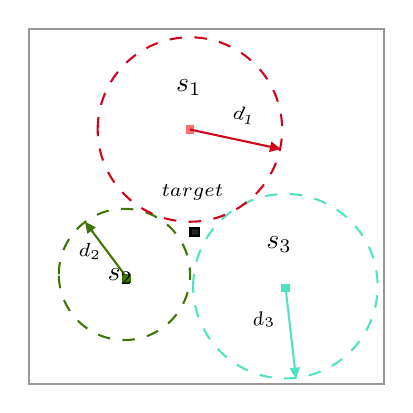
\begin{tikzpicture}[x=0.75pt,y=0.75pt,yscale=-1,xscale=1]
%uncomment if require: \path (0,300); %set diagram left start at 0, and has height of 300

%Shape: Square [id:dp9485406093696858] 
\draw  [color={rgb, 255:red, 154; green, 150; blue, 150 }  ,draw opacity=1 ] (314.5,50) -- (485.5,50) -- (485.5,221) -- (314.5,221) -- cycle ;
%Shape: Square [id:dp24929171411689466] 
\draw  [fill={rgb, 255:red, 33; green, 33; blue, 33 }  ,fill opacity=1 ] (392.46,146) -- (396.5,146) -- (396.5,150.04) -- (392.46,150.04) -- cycle ;
%Shape: Square [id:dp1889342057393233] 
\draw  [draw opacity=0][fill={rgb, 255:red, 80; green, 227; blue, 194 }  ,fill opacity=1 ] (436.14,173.04) -- (440.18,173.04) -- (440.18,177.08) -- (436.14,177.08) -- cycle ;
%Shape: Square [id:dp8116603792961381] 
\draw  [draw opacity=0][fill={rgb, 255:red, 248; green, 112; blue, 112 }  ,fill opacity=1 ] (390.14,96.54) -- (394.18,96.54) -- (394.18,100.58) -- (390.14,100.58) -- cycle ;
%Shape: Square [id:dp9501811324924574] 
\draw  [draw opacity=0][fill={rgb, 255:red, 65; green, 117; blue, 5 }  ,fill opacity=1 ] (359.6,168.36) -- (363.64,168.36) -- (363.64,172.4) -- (359.6,172.4) -- cycle ;
%Shape: Circle [id:dp3035334876106732] 
\draw  [color={rgb, 255:red, 65; green, 117; blue, 5 }  ,draw opacity=1 ][dash pattern={on 4.5pt off 4.5pt}] (329,168.38) .. controls (329,150.92) and (343.16,136.76) .. (360.62,136.76) .. controls (378.08,136.76) and (392.24,150.92) .. (392.24,168.38) .. controls (392.24,185.84) and (378.08,200) .. (360.62,200) .. controls (343.16,200) and (329,185.84) .. (329,168.38) -- cycle ;
%Shape: Circle [id:dp45289907486973524] 
\draw  [color={rgb, 255:red, 80; green, 227; blue, 194 }  ,draw opacity=1 ][dash pattern={on 4.5pt off 4.5pt}] (393.72,174.06) .. controls (393.72,149.52) and (413.62,129.62) .. (438.16,129.62) .. controls (462.7,129.62) and (482.6,149.52) .. (482.6,174.06) .. controls (482.6,198.6) and (462.7,218.5) .. (438.16,218.5) .. controls (413.62,218.5) and (393.72,198.6) .. (393.72,174.06) -- cycle ;
%Shape: Circle [id:dp28040021357673117] 
\draw  [color={rgb, 255:red, 208; green, 2; blue, 27 }  ,draw opacity=1 ][dash pattern={on 4.5pt off 4.5pt}] (347.72,98.56) .. controls (347.72,74.02) and (367.62,54.12) .. (392.16,54.12) .. controls (416.7,54.12) and (436.6,74.02) .. (436.6,98.56) .. controls (436.6,123.1) and (416.7,143) .. (392.16,143) .. controls (367.62,143) and (347.72,123.1) .. (347.72,98.56) -- cycle ;
%Straight Lines [id:da7421212837849427] 
\draw [color={rgb, 255:red, 208; green, 2; blue, 27 }  ,draw opacity=1 ]   (392.16,98.56) -- (433.15,107.37) ;
\draw [shift={(436.08,108)}, rotate = 192.13] [fill={rgb, 255:red, 208; green, 2; blue, 27 }  ,fill opacity=1 ][line width=0.08]  [draw opacity=0] (5.36,-2.57) -- (0,0) -- (5.36,2.57) -- cycle    ;
%Straight Lines [id:da6428590261529223] 
\draw [color={rgb, 255:red, 80; green, 227; blue, 194 }  ,draw opacity=1 ]   (438.16,174.06) -- (442.96,215.71) ;
\draw [shift={(443.31,218.69)}, rotate = 263.42] [fill={rgb, 255:red, 80; green, 227; blue, 194 }  ,fill opacity=1 ][line width=0.08]  [draw opacity=0] (5.36,-2.57) -- (0,0) -- (5.36,2.57) -- cycle    ;
%Straight Lines [id:da39676588633255805] 
\draw [color={rgb, 255:red, 65; green, 117; blue, 5 }  ,draw opacity=1 ]   (360.62,168.38) -- (343.4,145.38) ;
\draw [shift={(341.6,142.98)}, rotate = 53.17] [fill={rgb, 255:red, 65; green, 117; blue, 5 }  ,fill opacity=1 ][line width=0.08]  [draw opacity=0] (5.36,-2.57) -- (0,0) -- (5.36,2.57) -- cycle    ;


% Text Node
\draw (337.3,151.74) node [anchor=north west][inner sep=0.75pt]  [font=\scriptsize,rotate=-1.68] [align=left] {$\displaystyle d_{2}$};
% Text Node
\draw (420.08,185.84) node [anchor=north west][inner sep=0.75pt]  [font=\scriptsize,rotate=-351.95] [align=left] {$\displaystyle d_{3}$};
% Text Node
\draw (412.56,84.98) node [anchor=north west][inner sep=0.75pt]  [font=\scriptsize,rotate=-10.92] [align=left] {$\displaystyle d_{1}$};
% Text Node
\draw (377,123.5) node [anchor=north west][inner sep=0.75pt]  [font=\scriptsize] [align=left] {$\displaystyle target$};
% Text Node
\draw (427.5,148.5) node [anchor=north west][inner sep=0.75pt]   [align=left] {$\displaystyle s_{3}$};
% Text Node
\draw (351,164) node [anchor=north west][inner sep=0.75pt]   [align=left] {$\displaystyle s_{2}$};
% Text Node
\draw (384,73) node [anchor=north west][inner sep=0.75pt]   [align=left] {$\displaystyle s_{1}$};


\end{tikzpicture}